\documentclass[10pt]{article}
\usepackage[margin=0.8in]{geometry}
\usepackage{amsmath,amssymb,graphicx,hyperref}
\setlength{\parindent}{0pt}\setlength{\parskip}{7pt}
\begin{document}
\raggedright
\begin{center}{\Large Complete Lean proof: guarded fall-degree pair $(4,5)$}\\2026-10-29\end{center}

\textbf{Exact theorem.} \texttt{GuardedExactPair.exact\_pair\_prime} proves,
for every prime $p>3$, the ordinary first/last pair $(4,5)$ for the six inputs
\[
g(x),\ g(y),\ g(z),\ S_3(x,y,u),\ S_3(u,z,r),\ v(x-y)-1,
\quad g(T)=(T-a)(T-b)(T-c).
\]
The hypotheses are distinct $a,b,c$, nonzero $4\alpha^3+27\beta^2$, an
affine rational target, rational affine lifts for every base abscissa, and
no field assignment satisfying all six generators. The Semaev polynomial is
the explicit short-Weierstrass formula. Both degree predicates express
attainment and minimality. The unit ideal and degree-five refutation are
proved consequences.

\textbf{Last fall five.} The actual inputs reduce in degree four to two
quadratic families, using the missing-root state $w=a+b+c-x-y$.
Explicit cubic rotations and interpolation normalize the leading coefficients
through degree-five steps. Affine-grid identities extract a scalar resultant
through legal products and reductions. The second shifts may have degree
five; no degree-four bound for them is assumed.

Rational base lifts give the explicit first-quadratic roots
\[
\rho_\pm=\frac{(x+y)(xy+\alpha)+2\beta\ \pm2Z_xZ_y}{(x-y)^2}.
\]
This divides by no ordinate, including repeated roots and two-torsion.
The checked identity \texttt{quadRes\_split} expresses the scalar resultant
as the product of the second quadratic's values at these roots. Polynomial
UNSAT makes both values nonzero. An explicit nine-point interpolation inverse
then derives one in degree five by scalar-grid shifts. The checked separating
space excludes one in degree four. This proves the exact last-fall value,
including the rationality/unit-ideal bridge.

\textbf{First fall four.} The actual degrees $(3,3,3,4,4,2)$ and homogeneous
leading forms are proved. The degree-$d$ relation space and its classical
graded Koszul span use these actual polynomials. Every top relation below
four is zero. At four the witness
\[
(v,-v,0,0,0,-(x^2+xy+y^2))
\]
is nonzero and cannot be Koszul: every distinct pair of input degrees sums
to at least five. Its lift to the inhomogeneous inputs is nonzero and has
degree at most three. Thus the first fall is exactly four under the stated
ordinary homogeneous-top/Koszul convention.

\newpage
\begin{center}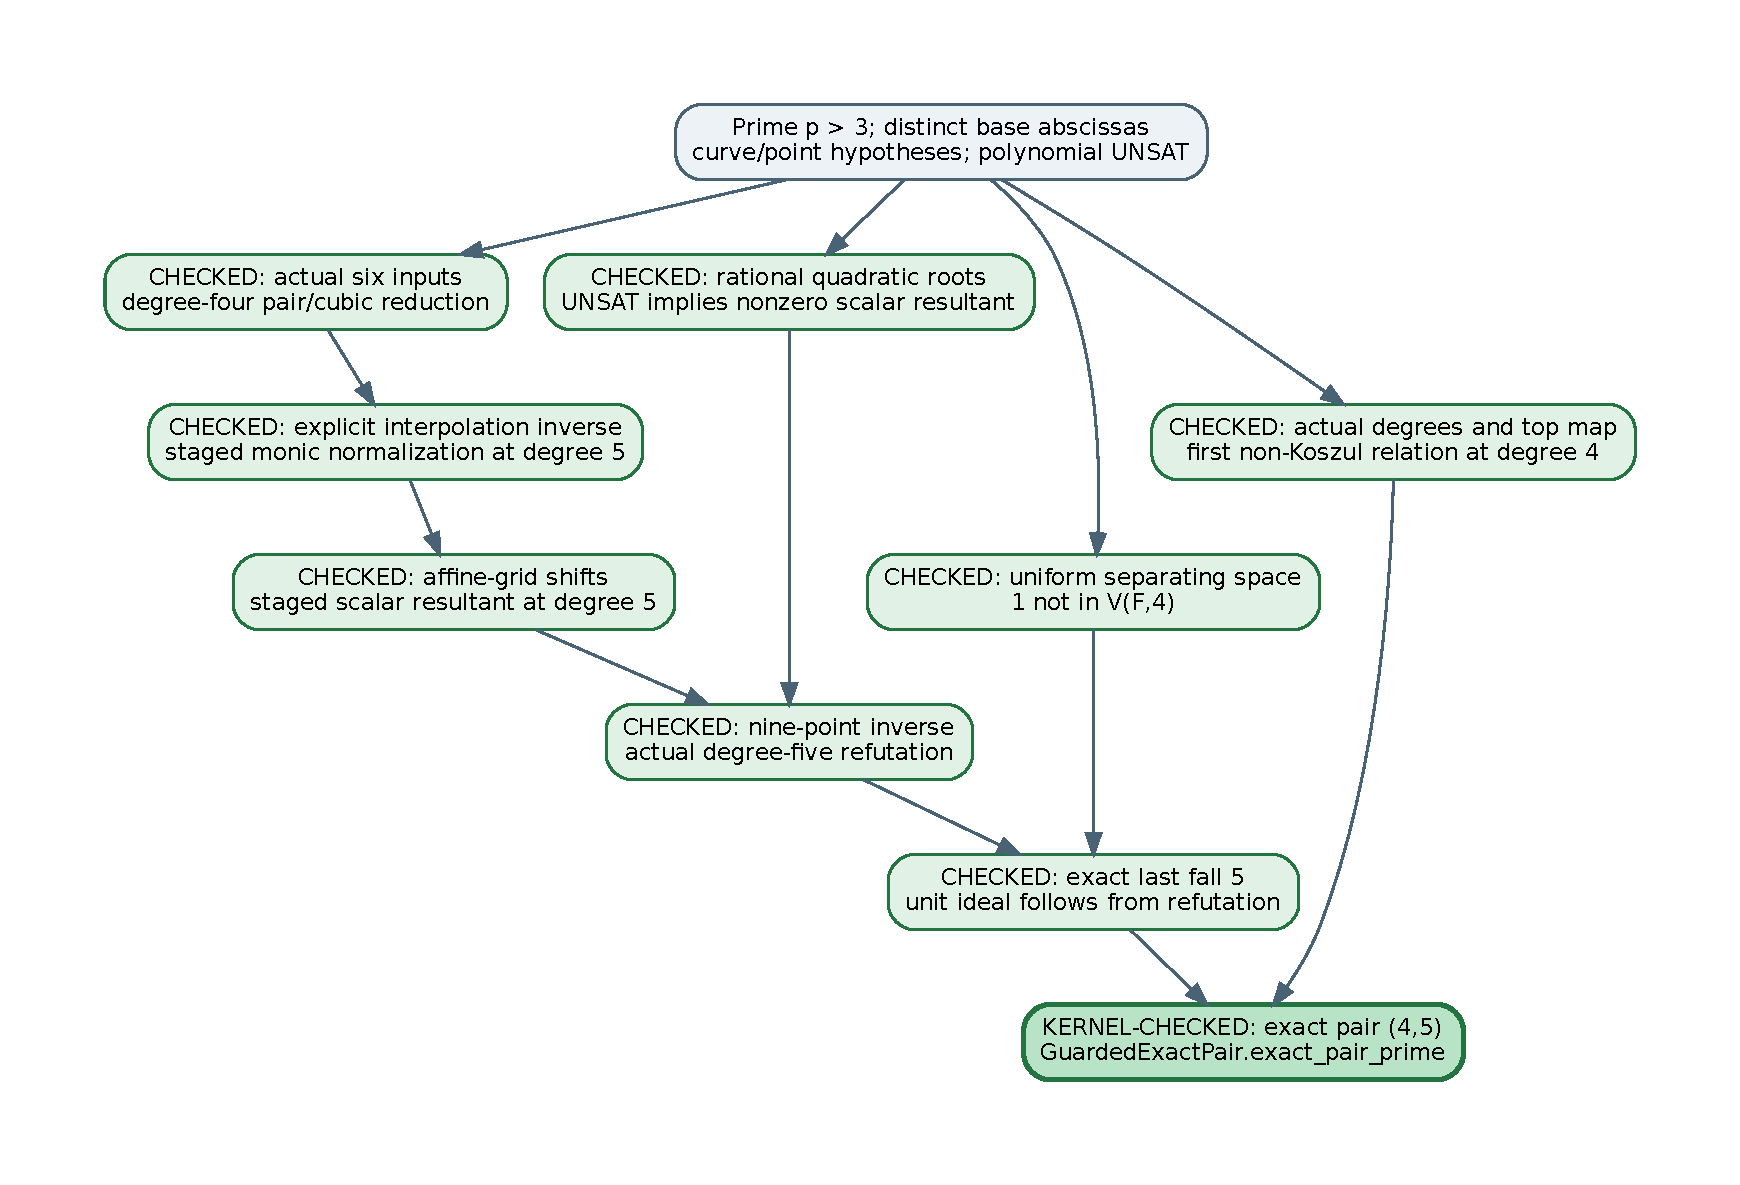
\includegraphics[width=0.98\linewidth,height=0.59\textheight,keepaspectratio]{complete-exact-pair-diagram.pdf}\end{center}

\textbf{Verification.} Pinned Lean4.34.1, Mathlib
\texttt{d13f23b723b8a846827a245b89c10fc7d3f11612}.
The default Lake build includes the final theorem and every dependency.
The transitive axiom audit accepts only \texttt{propext},
\texttt{Classical.choice}, \texttt{Quot.sound}; no custom axioms, placeholders,
compiler-trusted evaluation or kernel bypasses occur. Exact source hashes,
build/audit logs, individual fresh module replays and the library outcome
are retained in \path{complete-exact-pair-validation/}. Full statements
and reproduction commands are in \path{complete-exact-pair.md}.

\textbf{Scope.} The theorem is uniform in field size for this explicit
three-abscissa inverse-guarded ordinary-ring presentation. Growing bases,
characteristic-two and Boolean/Weil-descent statements remain separate.
It does not kernel-certify E12 runs or the standard-curve numerical witnesses.
No experiment sweep, timing, recovery, complexity or security claim is made.
Sources: HKYY1505.02532 (definitions), Caminata--Gorla2112.05579v2
(degree conventions), Semaev1504.01175 (S3), study audits and pinned Mathlib.
\end{document}
